\newpage
\section{Theoretische Grundlagen}

Der Grundaufbau und somit die leitende Idee des Geiger-Müller-Zählrohr ist der Kathodenzylinder % beschrieben in ... also REF hinzufügen
mit innen liegendem, axial verlaufendem Anodendraht mit der Funktion ein Elektrisches Feld durch einen Strom $U$ anzulegen.

\subsection{Elektrisches Feld}

Das resultierende Elektrische Fled ist durch den Aufbau radialysymetrisch, verhält sich also also an Orten mit gleichem Radius exakt gleich.
Beschrieben durch die Formel 

\begin{equation}  %vlt noch herleiten!!!
\label{eqn:efeld}
E(r) = \frac{U}{r \hspace{0.1cm} \text{ln} \left( \frac{r_k}{r_a} \right) }
\end{equation}

\begin{align*}
r_a = \text{Radius Anodendraht}     \hspace{1cm} r_k = \text{Radius Stahlmantel}
\end{align*}
Zu sehen ist hier, dass das Feld zwar radial abnimmt aber doch nur von einem Paramter $r$ abhängt. Hier also der Abstand vom Anodendraht.
Um die realistischen Bedingungen nicht zu verletzten, sollte festleget werden $r_a<r<r_k$.
Folglich ist die Spannung antipropotional zu $r$. Dies ermöglicht eine fast ungehinderte nährung an sehr hohe Feldstärken in der unmittelbaren Nähe des Drahtes, wenn also $r_a$ und somit $r$ klein genug ist. 

\subsection{Wechselwirkung einfallender Teilchen zum Elektrischen Feld} %maybe: 
Die für das Experiment interessante, einfallendende ionisierende Strahlung der radioaktiven Teilchen bewegt sich nun in den Zylinder unseres Zählrohrs.
Diese Strahlung kommt auf dem Weg durch das Gas in Kontakt mit Atomen bei denen Ionen und ELektronen herausgeschlagen werden. 
Nun befinden sich im Elektrischen Feld eine Kombination aus neutralen Atomen, positv geadene Ionen und die negativen ELektronen. 

\begin{figure} %maybe, auflösung tresh lol
  \centering
  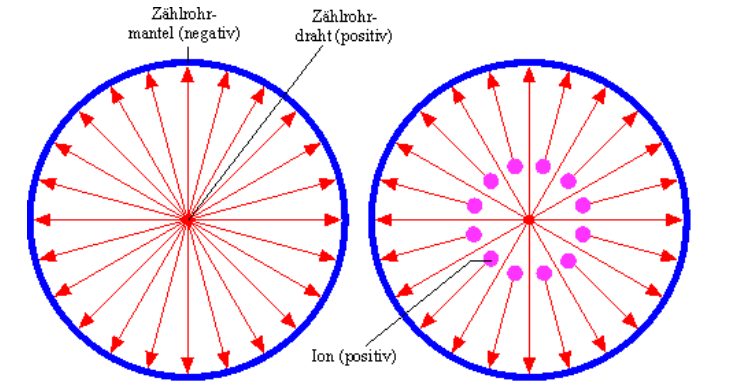
\includegraphics[width=0.7\textwidth]{bilder/Abbildung3.png}
  \caption{Orientierung des elektrischen Feldes \cite{leifi}.} 
  \label{fig:efeld}
\end{figure}

%vlt bild einfügen siehe ornder !!!!!!!!!!!!!!!!!!!!!!!!!!!!!!!!!!!!!!!!!!!!!!!!!!!!!!!!!!!!!!!!!
Das angelegte Feld führt dazu, dass sich die Ionene und ELektronen entsprechend ihrer Ladung entweder in Richtung des Stahlmantel (Ionen) oder zum Draht (Elektronen) bewegen.
Als \textbf{Ionisationsakt} bezeichnet man eben diesen Prozess, der solange anhält bis jegliche Energie der Strahlung durch Ionisation aufgebracht ist.
Die Energie der Teilchen Energie ferhält sich proportional zu Anzahl der enstandenen Elektronen und Ionen. 
\begin{equation}
\label{eqn:prop}
N \propto E
\end{equation}
Dabei ist N die Anzahl der Elektronen und Ionen und E die Energie des einfallenden Teilchens.
Was mit den abgeschlagen Teilchen der Gasatomen passiert hängt stark von dem Elektrischen Feld, also der angelegten SPannung, ab und lässt sich in 5 Stufen unterteilen.
Die Vorgänge unterscheiden sich für $\alpha$ - und $\beta$ - Teilchen lediglich in ihrem ausmaß der erzeugten Elektronen-Ionen-Paare, werden im folgenden also generalisiert dargestellt.
\paragraph{Abhängigkiet durch Spannung} \mbox{}

\subsubsection{Rekombination vor Sammlung}
\label{sub:Rekombination}
Bei sehr schwacher Spannung reicht die, durch das Elektrische Feld, generierte Beschleunigung auf die Elektronen nur selten aus um den Draht zu erreichen und einen Impuls zu erzeugen.
Der Hauptteil eben jener Elektronen wird durch \textbf{Rekombination}, ein Umkehrprozess der Ionisation, verhundert. Es liegt also anstelle eines Ionen und Elektronen wieder ein stabiles Gas Atom vor, unberührt vom Feld.
Diese Art der "Verschmelzung" braucht für seinen Teil auch Energie die durch den Stoß bei schwacher Spannung bereit gestellt wird.
\subsubsection{Ionisationskammer}
Ein erhötes Stromniveu führt zur sogenannten \textbf{Ionisationskammer}. Hier ist durch eine stärkere Beschleunigung durch das elektrische Feld die Wahrscheinlichkeit zur Rekombinationstark eingeschränkt und findet nur noch selten statt. 
Der Zusammenhang \eqref{eqn:prop} führt dazu, dass ein geringer Ionenstrom proportional zur Stromstärke entsteht.
Das Strahlungsteilchen löst also nun einen Strom an Ionen aus solange es sich mit ausreichend Energie durch den Zylinder bewegt. Vorraussetzung ist eine enstrpechende Länge des Zylinders, damit keine Energie verloren und somit nicht gemessen wird.
\subsubsection{Proportional-bereich}
\label{sub:porpotional}
Die nächste Erhöhung der Spannung würde eine noch schnellere Bewegung der Elektronen hervorrufen. Hier ist die Rekombination komplett ausgeschlossen, die Elektronen bewegen sich mit zu hoher Energie die nach \eqref{eqn:efeld} immer größer mit kleineren Abstand zum Draht wird.
Sobald ein beschleunigtes ELektron eine gewisse kinetische Energie erlangt ist es selbst in der Lage durch \textbf{Stoßionisation} andere Ionen und ELektronen aus den Gasatomen herauszulösen. Der Drahtnahen position zufolge werden diese auch stark beschleunigt und der Vorgang wiederholt sich
und wird \text{Townsend-Lawine} genannt. Es fallen also eine Vielzahl an Elektronen auf den Draht und es entsteht eine Ladung $Q$ die als \textbf{Ladungsimpuls} abgegriffen wereden kann. 
Immer noch gilt der Zusammenhang aus \eqref{eqn:prop}, da nur eben jene Elektronen Lawinen auslösen könenn, die nahe genug um Draht sind und wichtiger noch, selbst \textbf{direkt} durch die radioaktive Strahlung erzeugt worden sind. Dieser lässt sich erweitern zu
\begin{equation}
\label{eqn:prop2}
Q \propto E, I
\end{equation}
Die Ladungsimpulse geben also Aufschluss über die Energie und die Intensität $I$ der Teilchen. 
\subsubsection{Auslösebereich}
Erreicht die Spannung einen Wert der hoch genug ist verliert die Proportinalität ihre Bedeutung. 
Der Grund ist eine so hohe kinetisches Energie der Elektronen, dass beim Aufprall mit Gas Atomen zusätlich zu den ELektronen auch noch UV - Photonen erzeugt werden. 
Wärend die Elektronen weiterhin "Lawinen" %% ACHTUNG formation
in Richtung des Drahtes auslösen, sind die Photonen neutral geladen. Sie bewegen sich selbst mit ausreichend hoher Energie um Atome zu ionisieren aber sind unabhängig von 
Elektrischen Feldern. Durch diesen Sachverhalt entstehen nun im ganzen Zylinder eben diese Lawinen und das ursprünlgich durch Ionisation aufgetretende Elkektron verliert an Bedeutung.
Für den Fall reduziert sich also die Proportinalität der am Draht auftretenden Ladung auf
\begin{equation*}
\label{eqn:prop3}
Q \propto V, U, I
\end{equation*}
$V$ ist hier das Volumen des Zählerrohrs, also des Zylinders. $U$ bleibt weiterhin die angelegte Spannung und $I$ die Intensität.
Also ist hier keine Information mehr über die Energie der Strahlung selbst, sondern nur dessen Intensität.
Durch die nun im ganzen Zylinder auftretenden Lawinen ist der Ladungsimpuls jedoch stark erhöt und wesentlich leichter zu messen.

\subsection{Einfluss der positiven Ionen}
Es befinden sich also nun zwei Arten geladener Teilchen im Raum wobei ihre Massen sich unterscheiden
\begin{equation*}
\label{eqn:masse}
M_\text{Ion} >> M_\text{Elektron}
\end{equation*}
Nach Newton's zweitem Axiom wird die Beschleunigung eines Objektes maßgeblich durch ihre Masse beeinflussst
\begin{equation*}
\label{eqn:masse}
a= \frac{F}{m}
\end{equation*}
Die Kraft $F$ kommt vom Elektrischen Feld. Es folgt also aus \eqref{eqn:masse}, dass das Elektronen stärker beschleunigt wird. Eine Konsequenz daraus ist der \textbf{Ionenschlauch}. Dieser entseht 
durch einen längeren Aufenthalt der psotiven Ionen im Raum welche durch ihre Ladung ein eigenes positives Elektrisches Feld erzeugt. Die Richtung des durch die Spannung $U$ erzeugten Feldes ist nun genau dazu gegensetzlich.
\begin{equation*}
\label{eqn:Felder}
E_Z(r)\cdot \vec{e}_r + E_\text{Ionen}(r,t) \cdot \vec{e}_r = \vec{F}(r,t)
\end{equation*}
Die Differenz des vom Zählrohr $E_Z(r)\cdot \vec{e}_r$ und den Ionen $E_\text{Ionen}(r) \cdot \vec{e}_r$ ezreugtem Feld bildet nach dem Superpositionsprinzip  die Kraft $\vec{F}(r,t)$.
\subsubsection{Tod - und Erholungszeit}
Nun können Momente $\Delta T$ enstehen, in denen Die Kraft $\vec{F}(r,t)$ minimal wird, also auch die Elektronen in Richtung des Drahtes keine Beschleunigung mehr erfahren. 
Bei zu geringer Energie wird also trotz einfallender Strahlung Stoßionisation verhindert. Diesen Zeitraum $\Delta T$ nennt man \textbf{Totzeit}. Es entstehen keine Ladungsimpulse und dadurch kann kein Messwert der Intensität gefunden werden.
Durch Fehlende Stoßionisation bleibt aber auch die Generierung neue Ionen aus und der "Schlauch" bewegt sich in Richtung des Stahlmantels weg. 
In diesem Zeitraum der \textbf{Erholungszeit} $\Delta T_E$ lässt sich langsam wieder ein Ladungspuls feststellen der jedoch bis zur komplettten Abnahme des Schlauches abgeschwächt ist.

\paragraph{Bestimmung der Totzeit} 
\label{para:Totzeit}
\mbox{} \\
Da die Totzeit die Ladungsimpulsrate maßgeblich verringert gilt
\begin{equation*}
\label{ref:totzeitverhaeltnis}
N_r < N_w
\end{equation*}
Mit $N_r$ als gemessene Ladungsimpulsrate und $N_w$ als tatsächliche Ladungsimpulsrate. 
Letztere setzt sich zusammen aus der Impuslrate und der Messzeiet.
\begin{equation*}
\text{Impulsrate} = N_r \cdot t
\end{equation*} 
Also fehlt noch ein Quotient der der Impulsrate die korrektur durch die Totzeit beifügt. Dieser wird Messzeit genannt.
\begin{equation*}
\text{Messzeit} = (1-TN_r) \cdot t
\end{equation*}
Mit $T$ als Totzeit ist das also der Korrigierende Fakotor. $1-TN_r$ stelllt also den Teil der Zeit da, in der die Ionen die Manteldecke erreicht haben.
Final lässt sich die Ladungsimpulsrate bestimmmen 
\begin{equation}
\label{ref:Ladungsimpulsrate}
N_w = \frac{N_r}{1-TN_r}
\end{equation}
Dabei ist die Zählrate gemäß der Poisson-Statistik verteilt, somit lässt sich der Fehler auf die Zählrate gemäß $\sqrt{N}$
bestimmen.
\begin{equation}
\label{eqn:fehlerzählrate} %!!!!!!!!!!!!!!!!!!!!!!!!!!!!!!!!!!!!!!!!!!!!!!!!!!!!!!!!!!!!!!!!!!!!!!!!!!!!!!!!!!!!poisson HIER MORITZ
\increment N = \sqrt{N}
\end{equation}
Mit dieser Formel und einem weiteren radioaktiven Präperat  lässt sich die Totzeit berechnen. 
Durch messen von:\\
1.1)  $N_1$  \\
1.2) $N_{1+2}$\\
wobei $N_x$ die jeweilige Zählrate ist.
Aus dem Zusammenhang 
\begin{equation*}
N_{w1+2} = N_{w1} + N_{w2}
\end{equation*}
erhält man die Formel
\begin{equation*}
\frac{N_{1+2}}{1-TN_{1+2}}=\frac{N_1}{1-TN_1} + \frac{N_2}{1-TN_2}
\end{equation*}
nach $T$ umstellen
\begin{equation}
\label{eqn:totzeit}
T \approx \frac{N_1+N_2-N_{1+2}}{2N_1N_2}
\end{equation}


\subsubsection{Nachentladung}
\label{sub:Nachentladung}
Analog zu den Elektronen die eine Beschleunigung in Richtung des Drahtes erfahren, bewegen sich die Ionen entegegengesetz, hin zum Stahlmantel.
Auch wenn die Beschleunigung nach \eqref{eqn:masse} mehr zeit beanspruchen würede kommen sie mit Genug Energie an um Teilchen aus dem Stahl zum "schlagen", sogenannte \textbf{sekundär ELektronen}
Diese folgen wie die anderen \textbf{primär ELektronen} einer Bewegung in Richtung des Drahtes. Im Fall dass ein einziges Strahlungsteilchen würden diese sekundär ELektronen also verspätet zu den primären ankommen
und eine sogenannte \textbf{Nachentladung} erzeugen. Diese Verspätung wird durch $\Delta T_L$ ausgedrückt ud entspricht der Zeit die die positiven Ionen zum Mantel bennötigen.
Der Charakter der Totzeit verspricht, dass zu diesem Zeitpunkt($\Delta T_L$) der schlauch noch nicht den Stahlmantel erreicht hat. Also gilt
\begin{equation*}
\label{eqn:vergleich}
\Delta T < \Delta T_L
\end{equation*}

\subsection{Plateauzustände}
Bei konstanter Strahlungsintensität gegenüber der Spannung $U$ wird eine lineare Verteilung der Teilchen $N$ erkennbar. Dieser Abschnitt wird 
\textbf{Plateu} genannt. Das resultiert aus den Verschiedenen Spannungen und deren Einfluss auf die Messung. Bei niedriger Sappnung ist also noch Rekombination \ref{sub:Rekombination} möglcih und im späteren wir ddas Ergebnis durch Nachentladung \ref{sub:Nachentladung} verfälscht. 
Im Bereich des "Plateus" ist also annehmbar gute Messwerte zu bekommen. Durch nicht optimale Gasgemische lässt sich schon im Plateu einen linearen anstieg bekommen,
verschuldet durch trotzdem stattfindende Nachentladungen.


\subsection{Berechnung der Ladungsmenge im Zählrohr}
Durch die auschlagenden Elektronen entsteht auf dem Draht eine messbare Ladung die als Impuls weiterverarbeitet werden kann.
Diese Ladungsmenge kann gemittelt mit der bekannten Beziehung
\begin{equation*}
U=RI \hspace{2cm} I=\frac{U}{R}
\end{equation*}
und einer Mittellung mithilfe eines Integrals errechnet werden.
Der durchschnittlich fließende Strom $\si{\ampere}$ in einem Intervall von $0$ bis $\tau$ wobei gelten soll $\tau>>T$ wird dann ausgedrück durch
\begin{equation}
\label{eqn:ladungsmenge}
\bar{I} \coloneqq \frac{1}{\tau} \int_{0}^{\tau} \frac{U(t)}{R} \text{dt}
\end{equation}
Hier ist $R$ der auftrende Wiederstand.
%wenn relevant in den aufgaben auhc den zweiiten teil

\paragraph{frage von moritz} % titel duhhh
\mbox{}
\\ 
Der Versuch ist entsprechend der Anleitung mit einer 204Tl-Quelle aufgebaut. Die Quelle wurde so plaziert, dass bei einer mittleren Z¨ahlrohrspannung eine Z¨ahlrate von 100 Imp/s nicht
uberschritten wurde. Warum ist das wichtig?\\
idk\\
Bei einer höhern Zählrate würde die Bedingung der Totzeit verletzt werde. Wir würden teile des Intervalles in die Messung mit einbeziehn die nicht aussagend ist. In diesen nicht aussagenden Zeiten 
wird durch den Ionenschlauch das Feld im inneren maßgeblich verändert.
100 Imp/s ermöglicht möglich viele Messungen durch Impulsen, bei Berücksichtigung der Totzeit. Würde man die Totzeit verringern könenn wäre eine anpassung der Impulse pro Zeit möglich. Es folgt
\begin{equation*}
T \approx \frac{Imp}{sec}
\end{equation*}